\chapter{交流及其他损耗}
\section{引言}
尽管超导体的完美导电性让超导电性永恒迷住了科学家,诱惑了工程师和企业家,但适合做磁体的第II类超导体运行
于混合态,有磁滞损耗。第II类超导体在时变磁场、电流或两者同时存在的条件下本质上一定是有损耗的。
此外,当第II类超导体被处理成细丝嵌入正常金属基底这样的复合导体后,还会出现另一种磁损耗。
这些损耗通常称为交流损耗(AC~losses)。另外,磁体还有其他损耗,包括:1)导体接头;2) 洛伦兹力
导致的导体、绕组的移动,引发的摩擦热;3) 洛伦兹力导致的绕组浸渍破裂,也引起损耗。
尽管此处不会讨论,在聚变磁体中还存在另一种损耗:中子辐射。

耗散功率密度在第六章的方程6.1中用$g_d$表示,涵盖了出焦耳热外的所有损耗。
通常,它的大小和焦耳热密度$\rho_{cd}(T)J_{cd_o}^2(t)$相比是很小的。
虽然它幅值小,可它在绝热超导磁体,特别是LTS磁体中有关键作用,因为LTS磁体的稳态耗散基线应该是0或者接近0。
另一方面,第六章已经看到,绝热HTS磁体在其绕组内存在很大热耗散密度---示例中的高达$\sim 400\ \mathrm{kW/m^3}$,
尽管需要很大冷量---时仍能保持超导。
作为对比,水冷磁体的耗散密度基线可能是几十$\mathrm{GW/m^3}$;除了焦耳热之外的耗散基本都是可以忽略的。

第七章我们将讨论和研究三中类型的扰动项:1) 磁场相关的(交流损耗);2) 电场相关的(接头电阻);3) 机械相关的
(摩擦和环氧破裂)。对LTS磁体,交流损耗已被证实是具有严重危害的:仅有绕组“局域”的呗液氦冷却的---低温稳定---
LTS磁体才能承受交流损耗,这限制了它的应用范围(例如研究用、聚变用),基本上排除了商业相关的应用(从效率上讲,
绝热绕组更有优势)。仅有那些交流损耗可以容易降低的应用(例如直流应用,如NMR和MRI)是绝热LTS磁体可用且成功应用的。
随着交流损耗的可控和机械扰动的改善,多数绝热LTS NMR/MRI磁体大多数时间都能成功运行。
值得一说的是,如图6.1给出的扰动谱,在HTS磁体中,除了交流损耗外,没有重要的“不可约束”的扰动。
所以,第七章主要集中于交流损耗;接头损耗和机械扰动被视为“其他损耗”。

\section{交流损耗}
根据本书的基本哲学,只有那些可以用分析表达式计算粗略数的交流损耗例子才予以考虑;
即仅给出几个简单的例子来研究。
这样,一个复杂的“现实世界”的例子要么或者化简为分析可解模型---任何问题的推荐方法,要么在最开始就用代码求解---
不漂亮且缺少启发性的方法。

多丝复合超导体或股中的三种可区分交流损耗能量密$[\mathrm{J/m^3}]$为:1) 磁滞,$e_{hy}$;
2) 耦合,$e_{cp}$;3) 涡流,$e_{ed}$。
交流损耗由随时间变化的磁场和/或传输电流产生;此处仅考虑场电流激励。
置于某种场电流激励中,导体中的交流损耗取决于1)导体截面形状---此处考虑“Bean”板、圆柱、带---以及2)磁场相对于
导体轴的方向---要么长度方向,平行于宽面(如果有的话),要么垂直于它。

磁体绕组内的交流损耗增加了系统制冷负荷,因为HTS磁体运行温度远高于4.2 K,它能够容忍一些交流损耗。
对任何交流超导磁体而言,为了和室温磁体竞争,其总交流损耗乘以运行温度下的压缩机输入功率与热负荷的比值($W_{cp}/Q$)
必须要小于室温同类产品。
如图4.5可见,4.2 K时,$W_{cp}/Q$范围是250-8000,77 K时是10-50。
这些比率是交流超导磁体能否成功推向市场的主要指标。

第II类超导体的交流损耗研究自该类超导体用于磁体的1960年代末开始,一直持续到现在。
研究的基础已在1970年代和1980年代初期建立起来[1.27,7.1-7.16]。
最新的论文在合适的地方会被引用,包括HTS相关的。

\subsubsection*{超导体朝向与外磁场的关系}
如上所述,用于计算交流损耗的超导体截面包括:Bean板;圆(圆线)和长方形(代表带材)。
图7.1给出了这些导体置于空间均匀、时间变化的磁场$H_e(t)$中的情形:a) 宽为$2a$的Bean板;b)和c)直径为$d_f$的圆线;
d)和e)宽为$w$厚为$\delta$的带材。
注意到外场$H_e(t)$可能是圆线或带材取向三个方向中的任一个:沿圆线长度方向,为$H_{e\parallel}(t)$;
带材平行方向,为$H_{e\parallel}(t)$;圆线和带材垂直方向,为$H_{e\perp}(t)$。
对Bi2223和YBCO导体,仅能做成带材,交流损耗是严重的问题。

超导体中,传输电流仅在超导体轴向流过。传输电流被超导体的临界电流所限制。对Bean板,$I_c$是磁场方向单位板长度的值---
Bean板在场方向($y$轴)是无限长的,在电流方向($z$轴)的宽度是$2a$。
\begin{figure}[htbp]
	\centering
	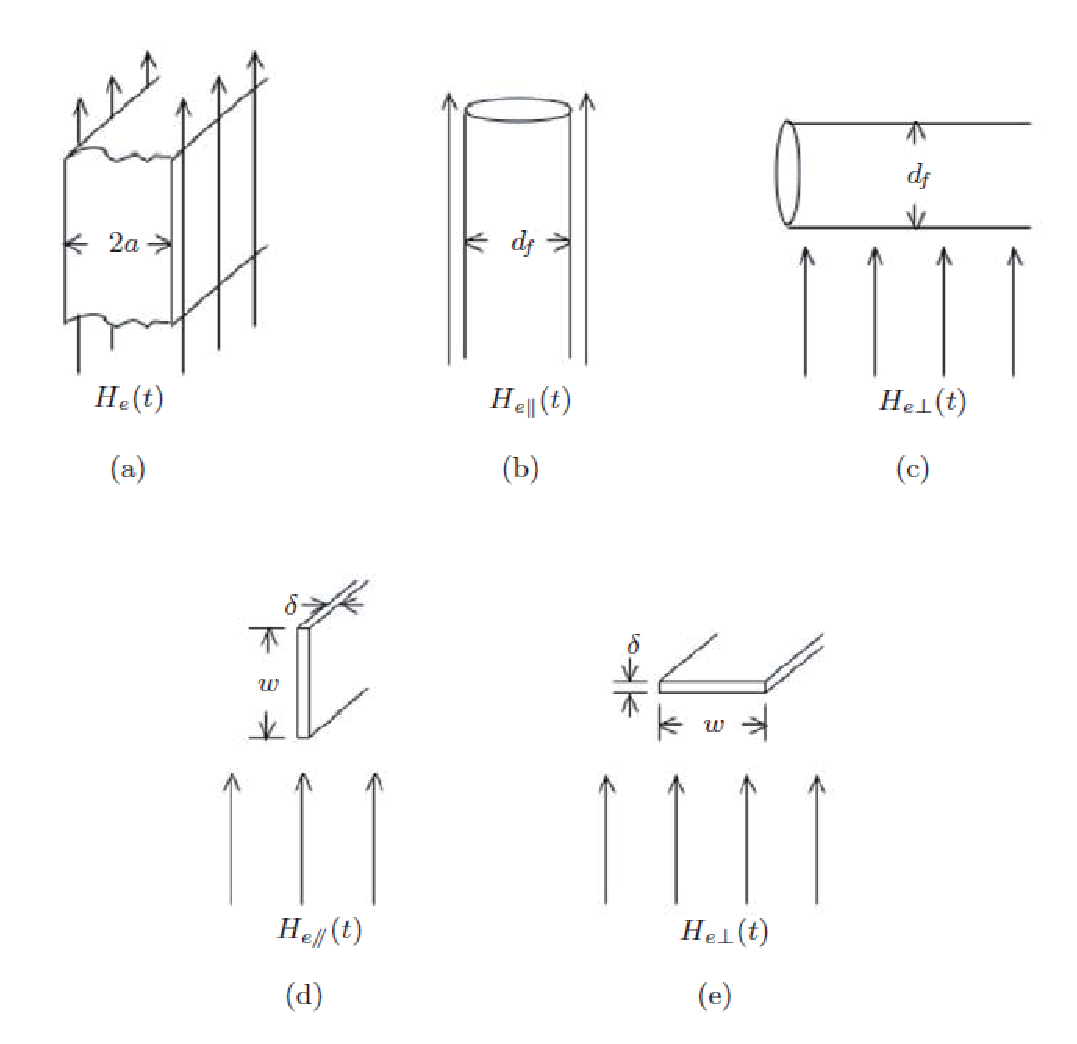
\includegraphics[scale=0.6]{chpt7/figs/fig7.1.eps}
	\caption{置于空间均匀时变磁场中的超导体。}
\end{figure}

\subsubsection*{时变磁场}
为了计算交流损耗,我们多数时候需要一个以磁场$H_m$或电流$I_m$最大幅值、频率$f$或周期$\tau_m$为变量的磁场或电流
的时间函数---如果频率多余一个,则$f$被视为主要频率。
“现实世界”的交流损耗非常复杂,即使采用程序也完全不可能精确的仿真问题,更别提交流损耗计算值的高精度了。
所以,建模为具有单一频率或周期的时间函数足够了,尤其是对粗略估算。

\subsubsection*{交流损耗的能量密度表}
交流损耗能量密度的闭式解析解总结如表7.3-7.9。表达式仅对图7.1给出的超导体配置和场方向有效;
对Bean板相关的表达式将在本章做推导。

\subsection{磁滞损耗}
如第二章所述,单位体积内的热耗散可以视为坡印廷矢量$\vec{S}$(方程2.20)流量。
积分形式下,忽略电能项,方程2.20成为:
\begin{equation}% 7.1
\int\left[-\int_{S}^{}\vec{E}\times\vec{H}\cdot d\vec{\ \mathcal{A}}\right]dt=\int_{\nu}^{}\left[\int\vec{E}\cdot\vec{J}dt+\frac{1}{2}\mu_oH^2+\mu_oH\int\vec{H}\cdot d\vec{M}\right]d\nu
\end{equation}
尽管Bean在他的第II类超导体磁场行为纯唯象(临界态模型)模型中使用了定义$\vec{B}=\mu_0(\vec{H}+\vec{M})$,
但如第五章所论及的,$B$是以超导体内磁场分布$H_s$下的“平均”磁感应强度$B_s$进行计算的,即$B_s(x)=\mu_0 H_s$。
因为Bean板仅在一个维度(x)上有限,$H_s(x)$和板内感应的超导电流密度$J_c$(Bean模型中,是依赖于场的)
仅在$x$方向变化。$J_c$是由电场$\vec{E}$建立起来的,后者是由$d\vec{B}(t)/dt$感应出来的。在Bean板中,
还可以写为均匀外磁场的时间变化率$\mu_0 d\vec{H_e}(t)/dt$。

\subsubsection*{Bean板的磁滞损耗}
所以,Bean的第II类超导体临界态模型中,$\vec{M}$是由$\vec{H_s}_x$表示的,后者又是由$\vec{J_c}$表示的。
相应的,宽度为$2a$的Bean板方程修改为:
\begin{equation}% 7.2
\int\left[-\int_{S}\vec{E}(x)\times\vec{H}_e\cdot d\vec{\ \mathcal{A}}\right]dt=\int_{0}^{2a}\left[\int\vec{E}(x)\cdot\vec{J}_c(x)dt+\frac{1}{2}\mu_oH_{s}^{2}(x)\right]dx
\end{equation}
式中,积分区间是$x=0$到$x=2a$(或者从$x=-a$到$x=a$)。
因为$\vec{J_c}(x)$是由$\vec{E}(x)$感应出的,所以它平行于$E$场。7.2中的$\int E(x)\cdot J_c(x)dt$表示的是
耗散,这个耗散被称为磁滞损耗。Bean板的磁滞损耗能量密度为:
\begin{equation}% 7.3a
e_{hy}=\frac{1}{2a}\int_{0}^{2a}\left[\int J_cE(x)dt\right]dx
\end{equation}
通过联立7.3和7.2,我们可以得到另一种表达式:
\begin{align*}% 7.3b
e_{hy}=\frac{1}{2a}\{\int\left[-\int_{S}\vec{E}(x)\times\vec{H}_e\cdot d\vec{\ \mathcal{A}}\right]dt-\frac{1}{2}\mu_oH\int_{0}^{2a}H_{s}^{2}(x)dx\} \tag{7.3'}
\end{align*}
方程7.3’表示板中的磁滞能量密度等于进入板的Poynting能量密度减去板中的磁能密度的总能量密度。

当外场$\vec{H}_e$经过一个完整周期,初始和终了磁场强度$\vec{H}_{e_i}$、$\vec{H}_{e_f}$
和磁化强度$\vec{M}(\vec{H}_{e_i})$和$\vec{M}(\vec{H}_{e_f})$都是相等的,$e_{hy}$于是还可以表示为:
\begin{equation}% 7.4a
e_{hy}=\mu_o\oint\vec{H}_ed\vec{M}_e(\vec{H}_e)
\end{equation}
从代数上看,上式还可以写为:
\begin{align*}% 7.4b
e_{hy}=-\mu_o\oint M(H_e)dH_e \tag{7.4'}
\end{align*}
在7.4’中,去掉了矢量符号。这是因为各矢量均仅有一个方向:$H_e$和$M$都是$y$向。

\subsubsection*{外磁场时间序列下的Bean板}
问题7.1-7.4和讨论7.1-7.2中,将研究Bean板置于外磁场在不同的时间序列下的磁滞能量密度。
情况1-6和情况1i-6i分别为板中无直流传输电流和有直流传输电流的情况,各情况由7.5定义。
\begin{equation}% 7.5
H_e(t)=0*(\ \mathrm{Virgin slab})\rightarrow H_m\rightarrow 0\rightarrow -H_m\rightarrow 0\rightarrow H_m\rightarrow 0\rightarrow -H_m\rightarrow 0
\end{equation}

简要描述方程7.5中给出的$H_e(t)$时间序列如下。
\begin{description}
	\item[情况1] $H_e(t)$从$0*$增加至$H_m$,其中$0*$表示板未经使用,即板中无超导电流密度$J_c$。
	\item[情况2] 这是情况1之后的场下降序列:$H_e(t)=H_m\rightarrow 0$。
	\item[情况3] 这是情况1和情况2的组合:$H_e(t)=0*\rightarrow H_m\rightarrow 0$。
	\item[情况4] 类似于情况1,但板已通过电流。
	\item[情况5] 类似情况2,但它紧随情况4:$H_e(t)=H_m\rightarrow 0$。
	\item[情况6] 开始于通过电流的的板,$H_e(t)$经过1个完整周期。
	\item[情况1i-6i] 除了一直同游直流传输电流,其他和对应的情况1-6一样。
\end{description}

情况1/2/4的$H_s(x)$图分别如图7.2-图7.4。没有传输电流时,板的磁场行为是关于中点$x=a$对称的;
因此,$H_s(x)$图仅给出$0\le x\le a$部分。情况1i-6i中的个别$H_s(t)$图后文给出。
\begin{figure}[htbp]
	\centering
	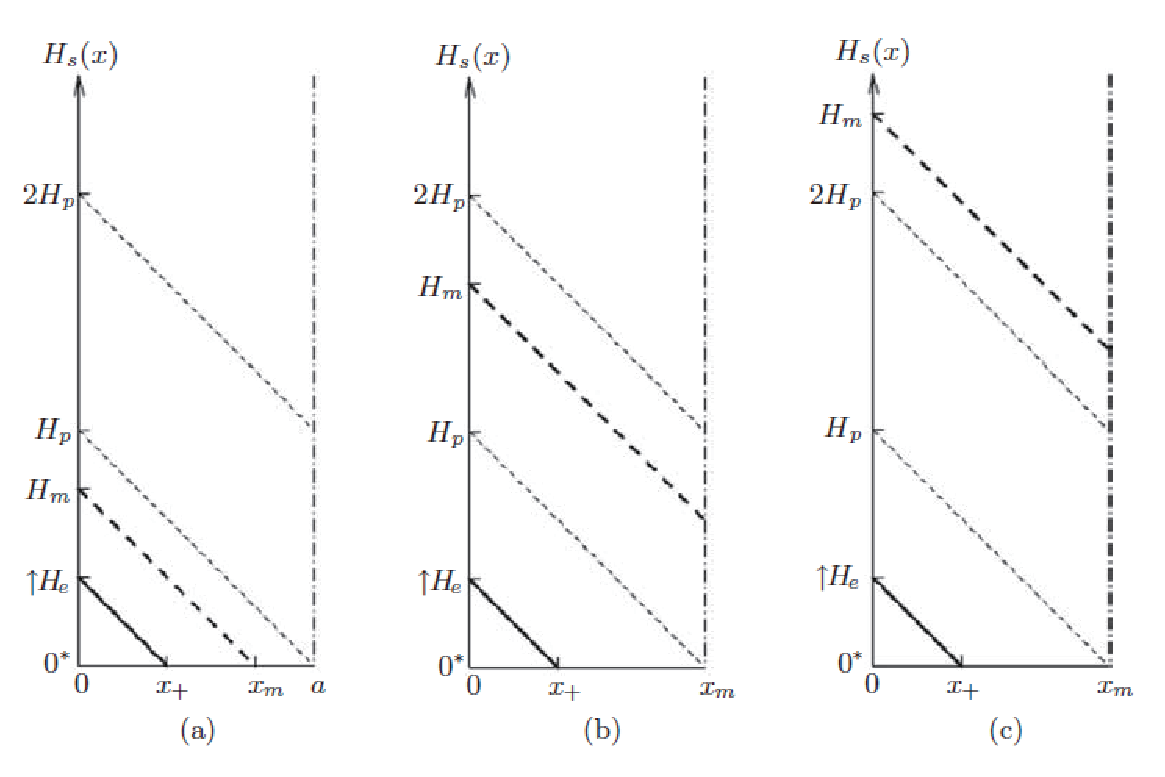
\includegraphics[scale=0.6]{chpt7/figs/fig7.2.eps}
	\caption{情况1的磁场特性。}
\end{figure}
\begin{figure}[htbp]
	\centering
	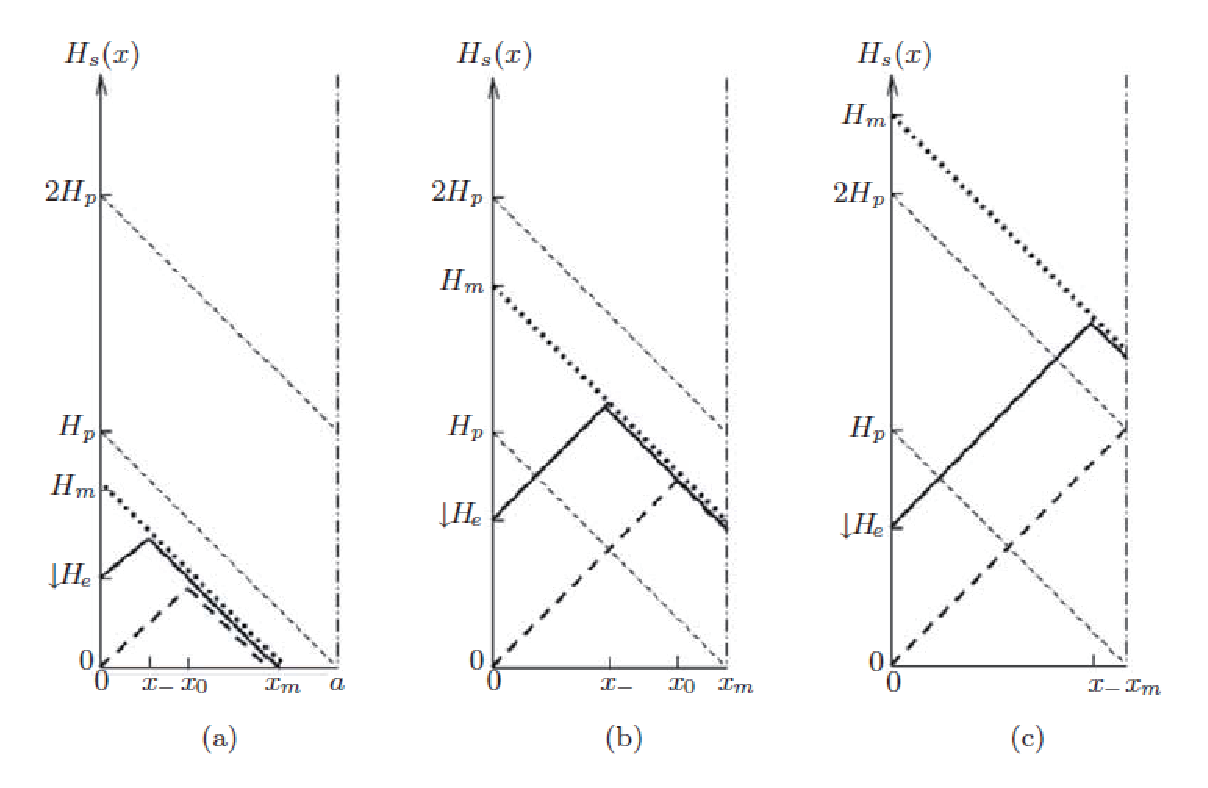
\includegraphics[scale=0.6]{chpt7/figs/fig7.3.eps}
	\caption{情况2的磁场特性。}
\end{figure}
\begin{figure}[htbp]
	\centering
	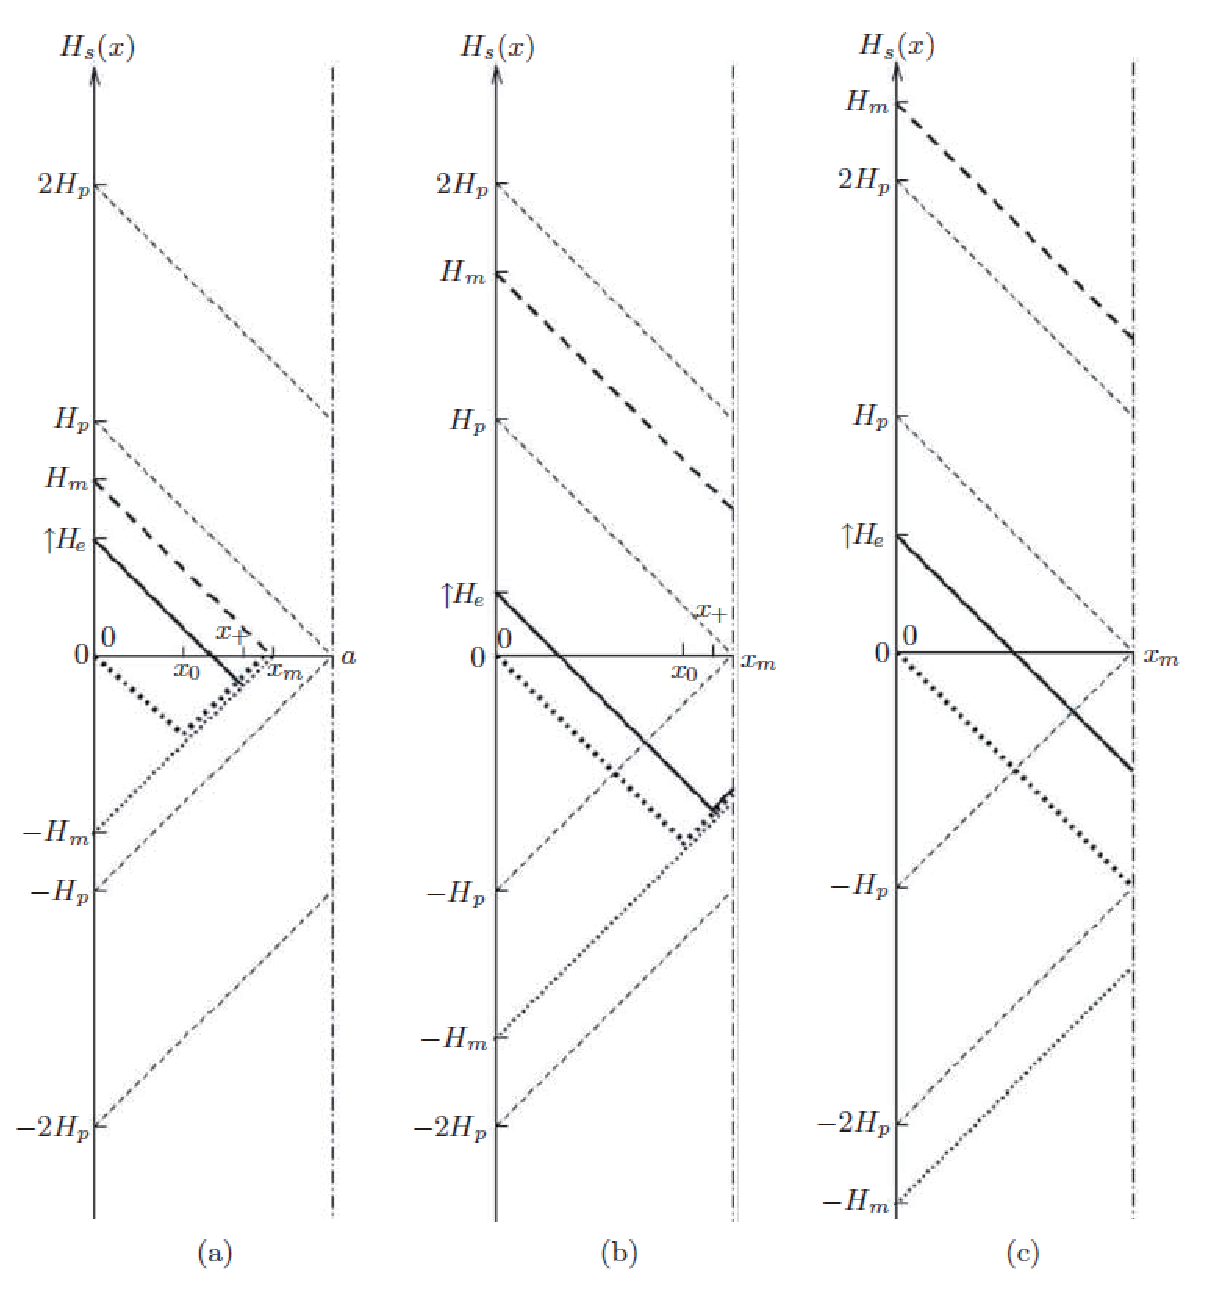
\includegraphics[scale=0.7]{chpt7/figs/fig7.4.eps}
	\caption{情况4的磁场特性。}
\end{figure}

\subsection{多丝复合物中的耦合损耗}
耦合损耗是多丝复合超导体中焦耳热的另一个形式,它来自时变外场在细丝之间感应出的耦合电流。
因为耦合电流通过金属基底金属,它随时间衰减。出于简单考虑,我们采用带有一个简单耦合时间常数$\tau_{cp}$
的指数模型。显然,$\tau_{cp}$越大,耦合电流在基底金属中流通的时间越长,造成的耦合能量损耗密度$e_{cp}$
越大。$\tau_{cp}$是耦合电流路径中电感$L$和电阻$R$的比值;$L/R$随着绕节距长度$\ell_p$的紧凑性增加而减小,
随基底金属电阻率增加而减少。图7.5给出了两根丝复合导体的示意图。多丝导体的复杂几何(比如换位丝就是复杂性的一个来源)
让基于Bean板的分析模型几乎不可能。
\begin{figure}[htbp]
	\centering
	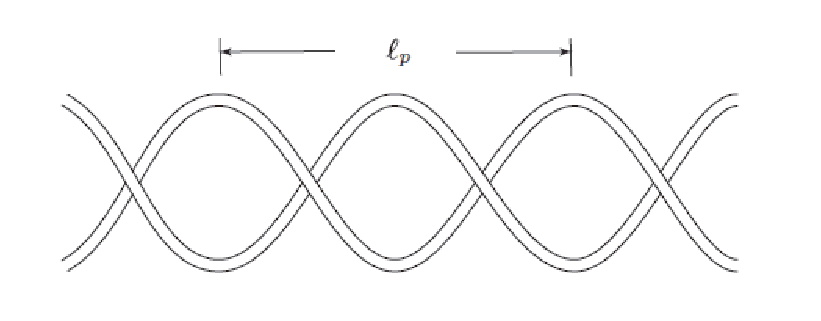
\includegraphics[scale=0.6]{chpt7/figs/fig7.5.eps}
	\caption{两根丝复合导体的示意图,使用方程7.6定义节距$\ell_p$。}
\end{figure}

\subsubsection*{耦合时间常数}
$e_{cp}$的关键参数是耦合时间常数$\tau_{cp}$。
它定义了多丝导体置于外时变场而感应出的丝间耦合电流的衰减时间常数。
实际中,电流衰减函数包括很多时间常数,不仅是主要的这一个。不过在实验中,
仅能确定主要的这一个,它被用于多数唯象方法中,$\tau_{cp}$定义为:
\begin{equation}% 7.6
\tau_{cp}=\frac{\mu_o\ell_{p}^{2}}{8\pi\rho_{ef}}
\end{equation}
式中,$\ell_p$是超导丝的节距,$\rho_{ef}$是丝间电流用到的有效基底电阻率。
如前所述,因为时间常数越长,能量耗散越大。故$\tau_{cp}$越大,$e_{cp}$越大。
正如Wilson指出[1.27]的,$e_{cp}$可以视为在复合导体内总磁能密度$\mu_0 H_m^2/2$的一部分,
当$\tau_{cp}\rightarrow 0$时有$e_{cp}\rightarrow 0$。
如前所述,有用的$e_{cp}$公式在表7.8给出;它包括了多丝线在四种外部磁场函数下的$e_{cp}$:1)
正弦;2)指数;3)三角波;4)梯形波。这些汉书的关键时间参数定义在图7.18中。

\subsubsection*{有效基底电阻}
我们将简要讨论方程7.5中出现的电阻率$\rho_{ef}$。它代表垂直于丝导体轴向的电流的基底有效电阻率。
Carr提出了两个模型[7.18]:
\begin{subequations}
	\begin{align}
	\rho_{ef0}&=\frac{1-\lambda_f}{1+\lambda_f}\rho_m\\
	\rho_{ef\infty}&=\frac{1+\lambda_f}{1-\lambda_f}\rho_m
	\end{align}
\end{subequations}
式中,$\lambda_f$是超导细丝在复合导体中的体积分数,$\rho_m$是基底的电阻率。

方程7.7a和7.7b基于图7.6中的两个极限电流分布:(a)中细丝表面的接触电阻是0,电流被拉入细丝中,令电路通路
的视在截面和距离分别变大和变小,故得到7.7a;(b)中恰好相反。
两个表达式都没有经受严格分析和试验的检验。实践中,方程7.7a和7.7b分别用于$\mathrm{Nb_3Sn}$和NbTi超导体的计算。

\subsection{涡流损耗}
涡流损耗的基本问题已在问题2.7中研究了。圆线(图7.1b和7.1c)和带材(图7.1d和7.1e)低频极限下的能量密度$e_{ed}$公式,总结如表7.9。
\begin{figure}[htbp]
	\centering
	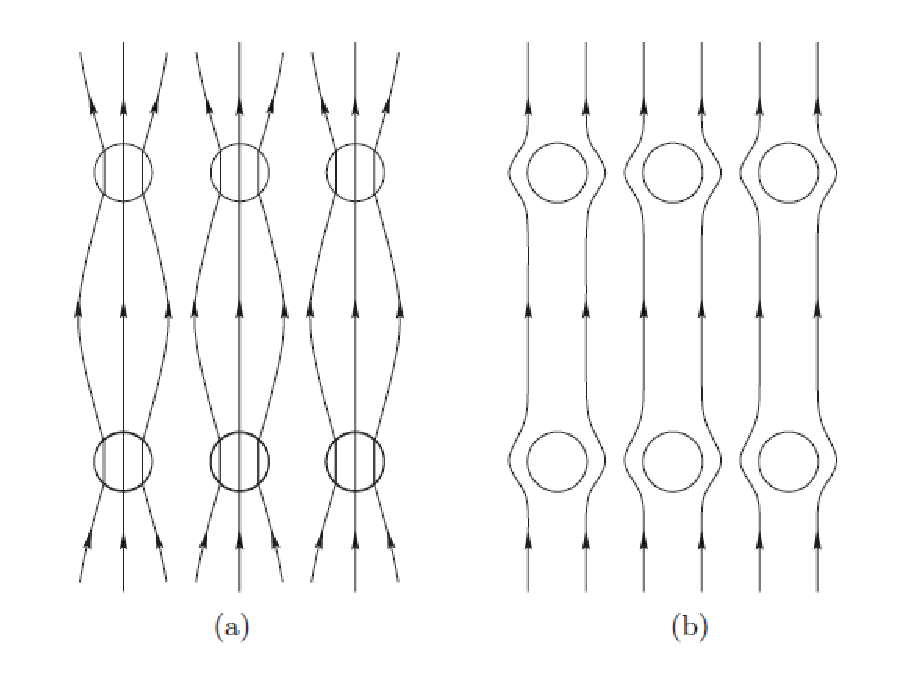
\includegraphics[scale=0.6]{chpt7/figs/fig7.6.eps}
	\caption{多丝超导体中垂直于导体轴的电流分布。}
\end{figure}

\section{其他损耗}
还有两个其他耗散源:1) 分段--或接头---电阻;和2) 机械扰动。
对于干式磁体的驱动模式,无论LTS还是HTS,必须将接头电阻处产生的损耗降至最低,原因很明显---它直接增加了制冷机的热负荷。
显然,这对持续运行模式的磁体不是问题---该模式要求接头近似为零,在$\mathrm{p\Omega}$数量级。
机械扰动---绕组内发生的导体运动或环氧浸渍绕组的环氧开裂---仅对“绝热”LTS磁铁重要;
对于冷却良好的LTS,最大的耗散源是复合超导体本身的焦耳热,机械扰动可以完全忽略。
处于一个不同的原因,如第6章所述,高HTS磁体,不论冷却良好或“绝热”,是不受这些机械扰动的影响的。
\subsection{接头电阻}
只有在以下情况下,电阻型接头才会成为设计问题:1)必须限制在受限空间内或遵从特定配置;
2)位于绕组内部较深的地方,那里的冷却有限或为零;3)必须承受较大的力;4)接头太多,其累积耗散会对系统的制冷负担加重。
5)不与制冷剂直接接触,如在低温冷却磁体中那样。

大致来讲,有两种类型接头:搭接接头和对接接头。
在大多数应用中,搭接接头比对接接头更好,原因有三个:1)比对接接头更容易制作;
2)通过简单增加搭接长度可以任意降低接头电阻;3)通常比对接接头更容易满足强度要求。
这里,我们讨论搭接拼接。

\subsubsection*{搭接电阻(接头)}
如图7.7所示,“握手式”搭接接头是最广泛使用的接头设计;它甚至非常适合在绕组内使用。
导线A和导线B之间的接头以搭接长度$\ell_{sp}$、宽度$a$和厚度$\delta_{sd}$经焊接而电气连接。
焊料电阻率为$\rho_{sd}$的焊料层电阻$R_{sd}$可由下式给出:
\begin{equation}% 7.8
R_{sd}=\frac{\rho_{sd}\delta_{sd}}{a\ell_{sp}}
\end{equation}
通常,$a$等于搭接导体的宽度。
\begin{figure}[htbp]
	\centering
	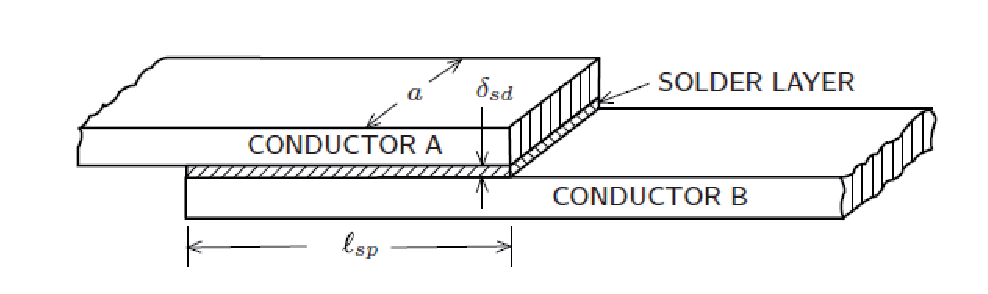
\includegraphics[scale=0.6]{chpt7/figs/fig7.7.eps}
	\caption{“握手式”搭接接头。}
\end{figure}

\subsubsection*{接触电阻}
\begin{equation}% 7.9a 7.9b
R_{sp}=R_{cA}+R_{sd}+R_{cB} 
=\frac{R_{ct}}{A_{ct}}
\end{equation}
\begin{equation}% 7.9c
R_{sp}=\frac{R_{ct}}{A_{ct}}\simeq R_{sd}
\end{equation}
\begin{equation}% 7.10
R_{ct}\simeq\rho_{sd}\delta_{sd}
\end{equation}


\subsubsection*{机械接触开关}

\subsection{机械扰动}

\subsubsection*{导体移动和矫正}
\begin{equation}% 7.11
e_f=\mu_ff_{L_r}\Delta r_f
\end{equation}
\begin{equation}% page411最后一个
\Delta r_f=\frac{e_f}{\mu_ff_{L_r}}=\frac{(1300\ \mathrm{J/m^3})}{(0.3)(2\times 10^8\ \mathrm{N/m^3})}\simeq 20\times 10^{-6}\ \mathrm{m}=20\ \mathrm{\mu m}
\end{equation}


\subsubsection*{填充材料分裂和矫正}

\section{声发射技术}
\subsection{机械事件探测——LTS磁体}

\subsection{应用于HTS磁体}




\section{专题}
\subsection{问题7.1:磁滞能量密度——在“小”磁场时间序列的“纯”Bean板}

\begin{equation}% 5.5
-M(H_e)=H_e-\frac{H_{e}^{2}}{2H_p}        (H_e=0*\rightarrow H_m\leq H_p)
\end{equation}
\begin{equation}% 7.12
-M(H_e)=H_e+\frac{H_{e}^{2}-2H_mH_e-H_{m}^{2}}{4H_p}      (H_e=H_m\rightarrow 0)
\end{equation}
\begin{equation}% 7.13a
e_{hy}=\frac{\mu_oH_{m}^{3}}{6H_p}        (0\leq H_m\leq H_p)
\end{equation}
\begin{equation}% 7.14a
e_{hy}=\frac{\mu_oH_{m}^{3}}{24H_p}       (0\leq H_m\leq H_p)
\end{equation}
\begin{equation}% 7.15a
e_{hy}=\frac{5\mu_oH_{m}^{3}}{24H_p}      (0\leq H_m\leq H_p)
\end{equation}

\subsubsection{问题7.1之解}
\begin{equation}% page416 1
E_z(x)=\mu_o\frac{dH_e}{dt}(x_+-x)
\end{equation}
\begin{equation}% page416 2
E_z(x)dt=\mu_o(x_+-x)dH_e
\end{equation}
\begin{equation}% page416 3 and 4
e_{hy}=\frac{1}{a}\int_{0}^{a}\left[\int J_cE(x)dt\right]dx 
=\frac{\mu_oF_c}{a}\int_{0}^{H_m}\left[\int_{0}^{x_+(x_+-x)dx}\right]dH_e
\end{equation}
\begin{equation}% page416 5 and 6
e_{hy}=\frac{\mu_oJ_c}{a}\int_{0}^{H_m}\left(x_{+}^{2}-\frac{x_{+}^{2}}{2}\right)dH_e 
=\frac{\mu_oJ_c}{a}\int_{0}^{H_m}\frac{H_{e}^{2}}{2J_{c}^{2}}dH_e=\frac{\mu_oH_{m}^{3}}{6aJ_c}
\end{equation}
\begin{equation}% 7.13a
e_{hy}=\frac{\mu_oH_{m}^{3}}{6H_p}    (H_m\leq H_p)
\end{equation}
\begin{equation}% page416 S1.3
E_z(x)dt=\mu_o(x-x_-)dH_e
\end{equation}
\begin{align*}% page416 S1.4
e_{hy}&=\frac{\mu_oJ_c}{a}\int_{H_m}^{0}\left[\int_{0}^{x_-}(x-x_-)dx\right]dH_e=\frac{\mu_oJ_c}{a}\int_{H_m}^{0}\left(\frac{x_{-}^{2}}{2}-x_{-}^{2}\right)dH_e \\\notag
&=\frac{\mu_oJ_c}{a}\int_{H_m}^{0}\frac{(H_m-H_e)^2}{8J_{c}^{2}}dH_e=\frac{\mu_oH_{m}^{3}}{24aJ_c}
\end{align*}
\begin{equation}% 7.14a
e_{hy}=\frac{\mu_oH_{m}^{3}}{24H_p}       (0\leq H_m\leq H_p)
\end{equation}
\begin{equation}% page417 S1.5a
E_z(0)=\mu_o\frac{H_e}{J_c}\left(\frac{dH_e}{dt}\right)
\end{equation}
\begin{equation}% page417 S1.6a两个
e_{py1}\equiv\frac{1}{a}\int\left[-\int_{S}\vec{E}(x)\times\vec{H}_e\cdot d\vec{\ \mathcal{A}}\right]dt=\frac{\mu_o}{aJ_c}\int_{0}^{H_m}H_{e}^{2}dH_e
e_{py1}=\frac{\mu_oH_{m}^{3}}{3H_p}
\end{equation}
\begin{equation}% page417 S1.5b
E_z(0)=-\mu_o\left(\frac{H_m-H_e}{2J_c}\right)\frac{dH_e}{dt}
\end{equation}
\begin{equation}% page417 S1.6b两个
e_{py2}=\frac{\mu_o}{2aJ_c}\int_{H_m}^{0}(H_m-H_e)H_edH_e
e_{py2}=-\frac{\mu_oH_{m}^{3}}{12H_p}
\end{equation}
\begin{equation}% page417 S1.7a
H_s(x)=J_cx        (0\leq x\leq x_0)
\end{equation}
\begin{equation}% page417 S1.7b
H_s(x)=H_m-J_cx    (x_0\leq x\leq H_m/J_c)
\end{equation}
\begin{equation}% page417 S1.8
e_{m_f}=\frac{\mu_o}{2a}\int_{0}^{a}H_{s}^{2}(x)dx=\frac{\mu_o}{2a}\left(2\times\int_{0}^{\frac{H_m}{2J_c}}J_{c}^{2}x^2dx\right)
e_{m_f}=\frac{\mu_oH_{m}^{3}}{24H_p}
\end{equation}
\begin{equation}% 7.15a两个
e_{hy}=e_{py1}+e_{py2}-e_{m_f} 
=\frac{\mu_oH_{m}^{3}}{3H_p}-\frac{\mu_oH_{m}^{3}}{12H_p}-\frac{\mu_oH_{m}^{3}}{24H_p}
e_{hy}=\frac{5\mu_oH_{m}^{3}}{24H_p}       (0\leq H_m\leq H_p)
\end{equation}
\begin{equation}% page418 S1.9
e_{py}=e_{hy}+e_{m_f}-e_{m_i}
\end{equation}


\begin{align*}% page418 S1.10两个
e_{m_{f1}}&=\frac{\mu_o}{2a}\int_{0}^{a}H_{s}^{2}(x)dx \\\notag
&=\frac{\mu_o}{2a}\left[\int_{0}^{\frac{H_m}{J_c}}(H_m-J_cx)^2dx\right]
\end{align*}
\begin{align*}
e_{m_{f1}}=\frac{\mu_oH_{m}^{3}}{6H_p}
\end{align*}



\begin{equation}% page418 S1.11a
e_{py1}=\frac{\mu_oH_{m}^{3}}{6H_p}+\frac{\mu_oH_{m}^{3}}{6H_p}=\frac{\mu_oH_{m}^{3}}{3H_p}
\end{equation}
\begin{equation}% page418 S1.11b
e_{py2}=\frac{\mu_oH_{m}^{3}}{24H_p}+\frac{\mu_oH_{m}^{3}}{24H_p}-\frac{\mu_oH_{m}^{3}}{6H_p}=\frac{\mu_oH_{m}^{3}}{12H_p}
\end{equation}


\subsection{问题7.2:磁滞能量密度——在“中”磁场时间序列的“纯”Bean板}


\begin{equation}% 5.5和5.6
-M(H_e)=H_e-\frac{H_{e}^{2}}{2H_p}                          (H_e=0*\rightarrow H_p)
=\frac{1}{2}H_p                                      (H_e=H_p\rightarrow H_m)
\end{equation}
\begin{equation}% 5.7a
-M(H_e)=\frac{1}{2}H_p-(H_m-H_e)+\frac{(H_m-H_e)^2}{4H_p}   (H_e=H_m\rightarrow 0)
\end{equation}
\begin{equation}% 7.13b
e_{hy}=\frac{1}{2}\mu_oH_pH_m\left(1-\frac{2H_p}{3H_m}\right)   (H_p\leq H_m\leq 2H_p)
\end{equation}
\begin{equation}% 7.15b
e_{hy}=\frac{1}{2}\mu_oH_pH_m\left[1-\frac{2H_p}{3H_m}+\frac{1}{12}\left(\frac{H_m}{H_p}\right)^2\right]     (H_p\leq H_m \leq 2H_p)
\end{equation}

\subsubsection{问题7.2之解}
\begin{equation}% page420 S2.1
e_{hy1^\prime}=\frac{1}{6}\mu_oH_{p}^{2}       (H_e=0\rightarrow H_p)
\end{equation}
\begin{equation}% page420 S2.2
E_z(x)=\mu_o\frac{dH_e}{dt}(a-x)
\end{equation}

\begin{subequations}
\begin{align*}% page420 S2.3a和2.3b
e_{hy1^\prime}&=\frac{1}{a}\int_{0}^{a}\left[\int J_cE(x)dt\right]dx=\frac{\mu_oJ_c}{a}\int_{0}^{a}\left[\int_{H_p}^{H_m}(a-x)dH_e\right]dx \\
&=\mu_oJ_c(H_m-H_p)\int_{0}^{a}\frac{a-x}{a}dx=\frac{1}{2}\mu_oH_p(H_m-H_p)
\end{align*}
\end{subequations}




\begin{equation}% page420 7.13b两个
e_{hy}=\frac{1}{6}\mu_oH_{p}^{2}+\frac{1}{2}\mu_oH_p(H_p-H_m) 
=\frac{1}{2}\mu_oH_pH_m-\frac{1}{3}\mu_oH_{p}^{2}
e_{hy}=\frac{1}{2}\mu_oH_pH_m\left(1-\frac{2H_p}{3H_m}\right)       (H_p\leq H_m\leq 2H_p)
\end{equation}
\begin{equation}% page420 S2.4a
e_{py1^\prime}=\frac{1}{3}\mu_oH_{p}^{2}
\end{equation}
\begin{equation}% page420 S2.5
E_z(0)=\mu_oa\frac{dH_e}{dt}
\end{equation}
\begin{equation}% page420 2.4b两个
e_{pyq^{\prime\prime}}\equiv\frac{1}{a}\int\left[-\int_{S}\vec{E}(x)\times\vec{H}_e\cdot d\vec{\ \mathcal{A}}\right]dt=\mu_o\int_{H_p}^{H_m}H_edH_e
e_{pyq^{\prime\prime}}=\frac{1}{2}\mu_o(H_{m}^{2}-H_{p}^{2})
\end{equation}
\begin{equation}% page421 S1.6b
e_{py2}=-\frac{\mu_oH_{m}^{3}}{12H_p}
\end{equation}
\begin{equation}% page421 S2.7两个
e_{m_f}=\frac{\mu_o}{2a}\int_{0}^{a}H_{s}^{2}(x)dx=\frac{\mu_o}{2a}\left[\int_{0}^{\frac{H_m}{2J_c}}J_{c}^{2}x^2dx+\int_{\frac{H_m}{2J_c}}^{a}(H_m-J_cx)^2dx\right]
e_{m_f}=\frac{1}{2}\mu_oH_{m}^{2}-\frac{\mu_oH_{m}^{3}}{8H_p}-\frac{1}{2}\mu_oH_mH_p+\frac{1}{6}\mu_oH_{p}^{2}
\end{equation}

\begin{align*}% page421 S2.8一个
e_{hy}&=e_{py1^\prime}+e_{py1^{\prime\prime}}+e_{py}-e_{m_f} \\\notag
&=\frac{1}{3}\mu_oH_{p}^{2}+\frac{1}{2}\mu_o(H_{m}^{2}-H_{p}^{2})-\frac{\mu_oH_{m}^{3}}{12H_p} 
-\left(\frac{1}{2}\mu_oH_{m}^{2}-\frac{\mu_oH_{m}^{3}}{8H_p}-\frac{1}{2}\mu_oH_mH_p+\frac{1}{6}\mu_oH_{p}^{2}\right) \\\notag
&=-\frac{1}{3}\mu_oH_{p}^{2}+\frac{\mu_oH_{m}^{3}}{24H_p}+\frac{1}{2}\mu_oH_pH_m \tag{S2.8}
\end{align*}

\begin{equation}% 7.15b
e_{hy}=\frac{1}{2}\mu_oH_pH_m\left[1-\frac{2H_p}{3H_m}+\frac{1}{12}\left(\frac{H_m}{H_p}\right)^2\right]     (H_p\leq H_m\leq 2H_p)
\end{equation}

\begin{equation}% 7.15a
e_{hy}=\frac{5\mu_oH_{m}^{3}}{24H_p}    (H_m\leq H_p) 
=\frac{5}{24}\mu_oH_{p}^{2}
\end{equation}

\begin{equation}% 7.15b
e_{hy}=\frac{1}{2}\mu_oH_pH_m\left[1-\frac{2H_p}{3H_m}+\frac{1}{12}\left(\frac{H_m}{H_p}\right)^2\right]    (H_p\leq H_m\leq 2H_p) 
=\frac{1}{2}\mu_oH_{p}^{2}\left[1-\frac{2}{3}+\frac{1}{12}\right]=\frac{5}{24}\mu_oH_{p}^{2}
\end{equation}


\subsection{问题7.3:磁滞能量密度——在“大”磁场时间序列的“纯”Bean板}

\begin{equation}% 7.16a
e_{hy2^\prime}=\frac{1}{3}\mu_oH_{p}^{2}
\end{equation}
\begin{equation}% 7.16b
e_{hy2^{\prime\prime}}=\frac{1}{2}\mu_oH_pH_m\left(1-\frac{2H_p}{H_m}\right)
\end{equation}
\begin{equation}% 7.14b
e_{hy}=\frac{1}{2}\mu_oH_pH_m\left(1-\frac{4H_p}{3H_m}\right)     (H_m\geq 2H_p)
\end{equation}
\begin{equation}% 7.15c
e_{hy}=\mu_oH_pH_m\left(1-\frac{H_p}{H_m}\right)      (H_m\geq 2H_p)
\end{equation}

\subsubsection{问题7.3之解}

\begin{equation}% 7.15b
e_{hy}=\frac{1}{2}\mu_oH_pH_m\left[1-\frac{2H_p}{3H_m}+\frac{1}{12}\left(\frac{H_m}{H_p}\right)^2\right]
=\mu_oH_{p}^{2}\left(1-\frac{1}{3}+\frac{4}{12}\right)=\mu_oH_{p}^{2}
\end{equation}
\begin{equation}% 7.15c
e_{hy}=\mu_oH_pH_m\left(1-\frac{H_p}{H_m}\right) 
=2\mu_oH_{p}^{2}\left(1-\frac{1}{2}\right)=\mu_oH_{p}^{2}
\end{equation}


\subsection{讨论7.1:磁滞能量密度——磁化的Bean板}

\begin{equation}% 7.17a
-M(H_e)=H_e-\frac{H_{e}^{2}+2H_mH_e-H_{m}^{2}}{4H_p}
\end{equation}
\begin{equation}% 7.17b
-M(H_e)=-\frac{1}{2}H_p+(H_m+H_e)-\frac{(H_m+H_e)^2}{4H_p}
\end{equation}
\begin{equation}% 5.6
-M(H_e)=\frac{1}{2}H_p
\end{equation}
\begin{equation}% 7.18
-M(H_e)=H_e+\frac{H_{e}^{2}+2H_mH_e-H_{m}^{2}}{4H_p}
\end{equation}


\begin{equation}% 5.7a
-M(H_e)=\frac{1}{2}H_p-(H_m-H_e)+\frac{(H_m-H_e)^2}{4H_p}
\end{equation}


\begin{equation}% 5.7b
-M(H_e)=-\frac{1}{2}H_p
\end{equation}


\begin{equation}% page425 S1.1b
E_z(x)dt=\mu_oH(x_+-x)dH_e
\end{equation}


\begin{equation}% page425 S1.2c
e_{hy}=\frac{\mu_oJ_c}{a}\int_{0}^{H_m}\left(x_{+}^{2}-\frac{x_{+}^{2}}{2}\right)dH_e
\end{equation}


\begin{equation}% 7.19a两个
e_{hy}=\frac{\mu_oJ_c}{2a}\int_{0}^{H_m}\left(\frac{H_m+H_e}{2J_c}\right)^2dH_e 
=\frac{\mu_o}{8H_p}\int_{0}^{H_m}(H_{m}^{2}+2H_mH_e+H_{e}^{2})dH_e
e_{hy}=\frac{7\mu_oH_{m}^{3}}{24H_p}
\end{equation}


\begin{equation}% page425 S2.2
E_z(x)=\mu_o\frac{dH_e}{dt}(a-x)
\end{equation}


\begin{equation}% 7.19b
e_{hy}=\frac{\mu_oJ_c}{2a}\left[\int_{0}^{2H_p-H_m}\left(\frac{H_m+H_e}{2J_c}\right)^2dH_e+\int_{2H_p-H_m}^{H_m}a^2dH_e\right] 
=\frac{\mu_o}{8H_p}\int_{0}^{2H_p-H_m}(H_{m}^{2}2H_mH_e+H_{e}^{2})dH_e+\frac{1}{2}\mu_oH_p\int_{2H_p-H_m}^{H_m}dH_e 
=\left(\frac{1}{3}\mu_oH_{p}^{2}-\frac{\mu_oH_{m}^{3}}{24H_p}\right)+(\mu_oH_pH_m-\mu_oH_{p}^{2})
e_{hy}=\mu_oH_pH_m\left[1-\frac{2H_p}{3H_m}-\frac{1}{24}\left(\frac{H_m}{H_p}\right)^2\right]      (H_p\leq H_m\leq 2H_p)
\end{equation}


\begin{equation}% 7.19c两个
e_{hy}=\frac{\mu_oJ_c}{2a}\left(\int_{0}^{H_m}a^2dH_e\right)=\frac{1}{2}\mu_oH_p\int_{0}^{H_m}dH_e
e_{hy}=\frac{1}{2}\mu_oH_pH_m      (H_m\geq 2H_p)
\end{equation}


\begin{equation}% 7.20a两个
e_{hy}=2\times7\left(\frac{7\mu_oH_{m}^{3}}{24H_p}+\frac{\mu_oH_{m}^{3}}{24H_p}\right)
e_{hy}=\frac{2\mu_oH_{m}^{3}}{3H_p}     (0\leq H_m\leq H_p)
\end{equation}


\begin{equation}% 7.4b和7.21
e_{hy}=\mu_o\oint-M(H_e)dH_e 
=2\mu_o\int_{0}^{H_m}-M(H_e)dH_e 
=2\mu_o\int_{0}^{H_m}\{-[M(H_e)]_{H_e=0\rightarrow H_m}+[M(H_e)]_{H_e=H_m\rightarrow 0}\}dH_e
\end{equation}

\begin{equation}% 7.20a两个
e_{hy}=2\mu_o\int_{0}^{H_m}\left[\left(H_e-\frac{H_{e}^{2}+2H_mH_e-H_{m}^{2}}{4H_p}\right) 
-\left(H_e+\frac{H_{e}^{2}-2H_mH_e-H_{m}^{2}}{4H_p}\right)\right]dH_e 
=2\mu_o\int_{0}^{H_m}\left(-\frac{H_{e}^{2}}{2H_p}+\frac{H_{m}^{2}}{2H_p}\right)dH_e=2\mu_o\left(-\frac{H_{m}^{3}}{6H_p}+\frac{H_{m}^{3}}{2H_p}\right)
e_{hy}=\frac{2\mu_oH_{m}^{3}}{3H_p}       (0\leq H_m\leq H_p)
\end{equation}


\begin{equation}% page427 前7.20b两个
e_{hy}=2\times\{\mu_oH_pH_m\left[1-\frac{2H_p}{3H_m}-\frac{1}{24}\left(\frac{H_m}{H_p}\right)^2\right]+\frac{\mu_oH_{m}^{3}}{24H_p}\}
e_{hy}=2\mu_oH_pH_m\left(1-\frac{2H_p}{3H_m}\right)        (H_p\leq H_m\leq 2H_p)
\end{equation}
\begin{equation}% 7.21
e_{hy}=-2\mu_o\int_{0}^{H_m}\{[M(H_e)]_{H_e=0\rightarrow H_m}-[M(H_e)]_{H_e=H_m\rightarrow 0}\}dH_e
\end{equation}
\begin{equation}% page427倒数第二个
e_{hy}=2\mu_o\{\int_{0}^{2H_p-H_m}\left[-\frac{1}{2}H_p+(H_m+H_e)-\frac{(H_m+H_e)^2}{4H_p}\right]dH_e 
+\int_{2H_p-H_m}^{H_m}\frac{1}{2}H_pdH_e-\int_{0}^{H_m}\left[\frac{1}{2}H_p-(H_m-H_e)+\frac{(H_m-H_e)^2}{4H_p}\right]\}dH_e
=2\mu_o\{\int_{0}^{2H_p-H_m}\left[-\frac{1}{2}H_p+H_m+H_e-\frac{H_{m}^{2}}{4H_p}-\frac{H_mH_e}{2H_p}-\frac{H_{e}^{2}}{4H_p}\right]dH_e 
+H_p(H_m-H_p)-\int_{0}^{H_m}\left[\frac{1}{2}H_p-H_m+H_e+\frac{H_{m}^{2}}{4H_p}-\frac{H_mH_e}{2H_p}+\frac{H_{e}^{2}}{4H_p}\right]\}dH_e 
=2\mu_o\left[\left(\frac{1}{3}H_{p}^{3}+\frac{1}{2}H_pH_m-\frac{1}{2}H_{m}^{2}+\frac{H_{m}^{3}}{12H_p}\right)\right] 
=2\mu_o\left(-\frac{2}{3}H_{p}^{2}+H_pH_m\right) 
e_{hy}=2\mu_oH_pH_m\left(1-\frac{2H_p}{3H_m}\right)       (H_p\leq H_m\leq 2H_p)
\end{equation}
\begin{equation}% page428 7.20c两个
e_{hy}=2\times\left[\frac{1}{2}\mu_oH_pH_m+\frac{1}{2}\mu_oH_pH_m\left(1-\frac{4H_p}{3H_m}\right)\right]
e_{hy}=2\mu_oH_pH_m\left(1-\frac{2H_p}{3H_m}\right)     (H_m\geq 2H_p)
\end{equation}
\begin{equation}% page428 7.21和7.20c合成的
e_{hy}=2\mu_o\int_{0}^{H_m}\{-[M(H_e)]_{H_e=0\rightarrow H_m}+[M(H_e)]_{H_e=H_m\rightarrow 0}\}dH_e 
=2\mu_o\{\int_{0}^{H_m}\frac{1}{2}H_pdH_e 
-\int_{H_m-2H_p}^{H_m}\left[\frac{1}{2}H_p-(H_m-H_e)+\frac{(H_m-H_e)^2}{4H_p}\right]-\int_{0}^{H_m-2H_p}(-\frac{1}{2}H_p)\}dH_e 
=2\mu_o\left[H_p(H_m-H_p) 
+\int_{H_m-2H_p}^{H_m}\left(-\frac{1}{2}H_p+H_m-\frac{H_{m}^{2}}{4H_p}-H_e+\frac{H_mH_e}{2H_p}-\frac{H_{e}^{2}}{4H_p}\right)dH_e\right] 
=2\mu_o[H_p(H_m-H_p)+\frac{1}{3}H_{p}^{2}]
e_{hy}=2\mu_oH_pH_m\left(1-\frac{2H_p}{3H_m}\right)       (H_m\geq 2H_p)
\end{equation}
\begin{equation}% 7.20d和7.20e
e_{hy}=2\mu_oH_pH_m   (H_m\gg H_p)
=2\mu_oJ_caH_m  (H_m\gg H_p)
\end{equation}

\subsection{讨论7.2:载有直流电流的Bean板}


\subsection{问题7.4:磁滞能量密度——载有直流电流的Bean板}
\begin{equation}% 7.22a
e_{hy}=\frac{7\mu_oH_{m}^{3}}{24H_p}      [0\leq H_m\leq H_p(1-i)]
\end{equation}
\begin{equation}% 7.22b
e_{hy}=\frac{\mu_oH_{m}^{3}}{24H_p}       [0\leq H_m\leq H_p(1-i)]
\end{equation}
\begin{equation}% 7.22c
e_{hy}=\frac{2\mu_oH_{m}^{3}}{3H_p}       [0\leq H_m\leq H_p(1-i)]
\end{equation}
\begin{equation}% 7.23a
e_{hy}=\frac{1}{2}\mu_oH_pH_m(1+i^2)      [H_m\geq2H_p(1-i)]
\end{equation}
\begin{equation}% 7.23b
e_{hy}=\frac{1}{2}\mu_oH_pH_m(1+i^2)-\frac{2}{3}\mu_oH_{p}^{2}(1-i^3)   [H_m\geq2H_p(1-i)]
\end{equation}
\begin{equation}% 7.23c
e_{hy}=2\mu_oH_pH_m(1+i^2)-\frac{4}{3}\mu_oH_{p}^{2}(1-i^3)     [H_m\geq2H_p(1-i)]
\end{equation}


\subsubsection{问题7.4之解}
\begin{equation}% page433 S4.1a
E_z(x)=\mu_o\frac{dH_e}{dt}(x_+-x)
\end{equation}
\begin{equation}% page433 S4.1b
E_z(x)dt=\mu_o(x_+-x)dH_e
\end{equation}
\begin{equation}% 7.3a和S4.2a
e_{hyx}=\frac{1}{2a}\int_{0}^{a}\left[\int J_cE(x)dt\right]dx
=\frac{\mu_oJ_c}{2a}\int_{0}^{H_m}\left[\int_{0}^{x_+}(x_+-x)dx\right]dH_e
\end{equation}
\begin{equation}% page433 S4.2b
e_{hyx}=\frac{7\mu_oH_{m}^{3}}{48H_p}
\end{equation}
\begin{equation}% 7.22a
e_{hy}=\frac{7\mu_oH_{m}^{3}}{24H_p}      [0\leq H_m\leq H_p(1-i)]
\end{equation}
\begin{equation}% page433 S4.3a
e_{hyx}=\frac{\mu_oJ_c}{2a}\int_{H_m}^{0}x_{+}^{2}dH_e=-\frac{\mu_o}{16H_p}(H_m-H_e)^2dH_e 
=\frac{\mu_oH_{m}^{3}}{48H_p}
\end{equation}
\begin{equation}% 7.22b
e_{hy}=\frac{\mu_oH_{m}^{3}}{24H_p}        [0\leq H_m\leq H_p(1-i)]
\end{equation}
\begin{equation}% page434 S4.4
3_{hy}=2\times\left(\frac{7\mu_oH_{m}^{3}}{24H_p}+\frac{\mu_oH_{m}^{3}}{24H_p}\right)
\end{equation}
\begin{equation}% 7.22c
e_{hy}=\frac{2\mu_oH_{m}^{3}}{3H_p}         [0\leq H_m\leq H_p(1-i)]
\end{equation}
\begin{equation}% page434 S4.5a
e_{hyx}=\frac{\mu_oJ_c}{2a}\int_{0}^{H_m}\left[\int_{0}^{\ell^*}(\ell^*-x)dx\right]dH_e
\end{equation}
\begin{equation}% page434 S4.5b
e_{hyx}=\frac{\mu_oJ_ca^2(1-i)^2}{4a}\int_{0}^{H_m}dH_e=\frac{1}{4}\mu_oH_pH_m(1-i)^2
\end{equation}
\begin{equation}% page434 S4.6a
e_{hy\xi}=\frac{\mu_oJ_c}{2a}\int_{0}^{H_m}\left[\int_{0}^{\ell^*}(\ell^*-\xi)d\xi\right]dH_e
\end{equation}
\begin{equation}% page434 S4.6b
e_{hy\xi}=\frac{\mu_oJ_ca^2(1+i)^2}{4a}\int_{0}^{H_m}dH_e=\frac{1}{4}\mu_oH_pH_m(1+i)^2
\end{equation}
\begin{equation}% 7.23a
e_{hy}=\frac{1}{2}\mu_oH_pH_m(1+i^2)    [H_m\geq 2H_p(1-i)]
\end{equation}
\begin{equation}% page434 S4.7a
e_{hyx}=\frac{\mu_oJ_c}{2a}\int_{H_m}^{H_{m}^{*}}\left[\int_{0}^{x_+}(x-x_+)dx\right]dH_e
\end{equation}


\begin{align*}% page434 S4.7b
e_{hyx}&=\frac{\mu_oJ_c}{2a}\int_{H_{m}^{*}}^{H_m}\left(\frac{H_m-H_e}{2J_c}\right)^2dH_e \\
&=\frac{\mu_o}{16H_p}(H_{m}^{2}H_e-H_mH_{e}^{2}+\frac{1}{3}H_{e}^{3})\mid_{H_m-2H_p(1-i)}^{H_m} \\
&=\frac{1}{6}\mu_oH_{p}^{2}(1-i)^3
\end{align*}

\begin{equation}% page435 S4.7c
e_{hy}=\frac{1}{3}\mu_oH_{p}^{2}(1-i)^3
\end{equation}

\begin{align*}% page435 S4.8a
e_{hyx}&=\frac{\mu_oJ_c}{2a}\int_{H_{m}^{*}}^{0}\left[\int_{0}^{x_+}(x-x_+)dx\right]dH_e=-\frac{\mu_oH_p(1+i)^2}{4}\int_{H_{m}^{*}}^{0}dH_e \\
&=\frac{1}{4}\mu_oH_p(1+i)^2[H_m-2H_p(1-i)] \\
&=\frac{1}{4}\mu_oH_pH_m(1+i)^2-\frac{1}{2}H_{p}^{2}(1+i)^2(1-i)
\end{align*}

\begin{equation}% page435 S4.8b
e_{hy\xi}=\frac{1}{4}\mu_oH_pH_m(1-i)^2-\frac{1}{2}H_{p}^{2}(1-i)^3
\end{equation}
\begin{equation}% pge435 S4.8c
e_{hy}=\frac{1}{2}\mu_oH_pH_m(1+i^2)-\mu_oH_{p}^{2}(1-i)(1+i^2)
\end{equation}
\begin{equation}% 7.23b
e_{hy}=\frac{1}{2}\mu_oH_pH_m(1+i^2)-\frac{2}{3}\mu_oH_{p}^{2}(1-i^3)     [H_m\geq H_p(1-i)]
\end{equation}
\begin{equation}% page435 S4.9
e_{hy}=2\times\left[\frac{1}{2}\mu_oH_pH_m(1+i^2)+\frac{1}{2}\mu_oH_pH_m(1+i^2)-\frac{2}{3}\mu_oH_{p}^{2}(1-i^3)\right]
\end{equation}
\begin{equation}% 7.23c
e_{hy}=2\mu_oH_pH_m(1+i^2)-\frac{4}{3}\mu_oH_{p}^{2}(1-i^3)     [H_m\geq H_p(1-i)]
\end{equation}
\begin{equation}% page435 S4.10
e_{hy}=2\mu_oH_pH_m-\frac{4}{3}\mu_oH_{p}^{2}
\end{equation}
\begin{equation}% page435 7.20b
e_{hy}=2\mu_oH_pH_m\left(1-\frac{2H_p}{3H_m}\right)
\end{equation}


\subsection{问题7.5:自场磁滞能量密度——Bean板}
\begin{equation}% 7.25
I(t)=0^*(\ \mathrm{Virgin slab})\rightarrow I_m\rightarrow 0\rightarrow -I_m\rightarrow 0\rightarrow I_m\rightarrow 0\rightarrow -I_m\rightarrow 0
\end{equation}
\begin{equation}% 7.26a
e_{sf}=\frac{7}{24}\mu_oH_{p}^{2}i_{m}^{3}
\end{equation}
\begin{equation}% 7.26b
e_{sf}=\frac{1}{24}\mu_oH_{p}^{2}i_{m}^{3}
\end{equation}
\begin{equation}% 7.26c
e_{sf}=\frac{2}{3}\mu_oH_{p}^{2}i_{m}^{3}
\end{equation}

\subsubsection{问题7.5之解}
\begin{align*}% page437 S5.1a和S5.1b
e_{sfx}&=\frac{\mu_oJ_c}{2a}\int_{0}^{-H_pi_m}\left[\int_{0}^{x_+}(x-x_+)dx\right]dH_{sf} \\
&=\frac{\mu_oJ_c}{4a}\int_{0}^{-H_pi_m}(-x_{+}^{2})dH_{sf}
\end{align*}

\begin{equation}% page437 S5.2a和5.2b
e_{sfx}=\frac{\mu_oH_{p}^{2}}{16}\int_{0}^{i_m}(i_{m}^{2}+2i_mi+i^2)di 
=\frac{7}{48}\mu_oH_{p}^{2}i_{m}^{3}
\end{equation}

\begin{equation}% 7.26a
e_{sf}=\frac{7}{24}\mu_oH_{p}^{2}i_{m}^{3}
\end{equation}


\begin{align*}% page437 S5.3a和S5.3b和S5.3c
e_{sfx}&=\frac{\mu_oJ_c}{2a}\int_{-H_pi_m}^{0}\left[\int_{0}^{x_+}(x_+-x)dx\right]dH_{sf} \\
&=\frac{\mu_oH_{p}^{2}}{16}\int_{i_m}^{0}(i_{m}^{2}-2i_mi+i^2)di \\
&=\frac{1}{48}\mu_oH_{p}^{2}i_{m}^{3}
\end{align*}


\begin{equation}% 7.26b
e_{sf}=\frac{1}{24}\mu_oH_{p}^{2}i_{m}^{3}
\end{equation}
\begin{equation}% page437 S5.4
e_{sf}=2\times\left(\frac{7}{24}\mu_oH_{p}^{2}i_{m}^{3}+\frac{1}{24}\mu_oH_{p}^{2}i_{m}^{3}\right)
\end{equation}
\begin{equation}% 7.26c
e_{sf}=\frac{2}{3}\mu_oH_{p}^{2}i_{m}^{3}
\end{equation}


\begin{equation}% page438 7.20a和7.26c
e_{hy}=\frac{2\mu_oH_{m}^{3}}{3H_p} 
=\frac{2\mu_o(H_pi_m)^3}{3H_p} 
=\frac{2}{3}\mu_oH_{p}^{2}i_{m}^{3}
\end{equation}


\subsection{讨论7.3:磁体整体的交流损耗}


\subsection{讨论7.4:测量交流损耗的技术}




\subsection{讨论7.5:CICC中的交流损耗}



\subsection{讨论7.6:HTS中的交流损耗}




\subsection{问题7.6:$Nb_3Sn$中的磁滞损耗}


\subsubsection{问题7.6之解}
\begin{align*}% page448第一个
J_c(0\ \mathrm{T},4.2\ \mathrm{K})&=J_c(3\ \mathrm{T},4.2\ \mathrm{K})\times\left| \frac{M(0\ \mathrm{T},4.2\ \mathrm{K})}{M(3\ \mathrm{T},4.2\ \mathrm{K})}\right| \\ 
&\simeq J_c(3\ \mathrm{T},4.2\ \mathrm{K})\times\frac{(0.47\ \mathrm{T})}{(0.12\ \mathrm{T})}\\
&\simeq J_c(3\ \mathrm{T},4.2\ \mathrm{K})\times 3.92 \\
&\simeq 2.8\times 10^{10}\ \mathrm{A/m^2}
\end{align*}


\begin{equation}% page448第二个
M(H)=\frac{1}{2}H_p=\frac{1}{2}(d_{eff}/2)J_c(H)
\end{equation}

\begin{align*}% page448第三个
d_{eff}=\frac{4\mu_oM(0\ \mathrm{T})}{\mu_oJ_c(0\ \mathrm{T})}&\simeq\frac{4(470\times 10^{-3}\ \mathrm{T})}{(4\pi\times 10^{-7}\ \mathrm{H/m})(2.8\times10^{10}\ \mathrm{A/m^2})}\\
&=53\ \mathrm{\mu m}
\end{align*}

\begin{equation}% page488 5.40
a_c=\sqrt{\frac{3\tilde{C}_s(T_c-T_{op})}{\mu_oJ_{c_o}^{2}}}
\end{equation}
\begin{equation}% page488 S6.1
aJ_{c_o}\leq\sqrt{\frac{3\tilde{C}_s(T_c-T_{op})}{\mu_o}}
\end{equation}


\subsection{问题7.7:混合III SCM中的交流损耗}




\subsubsection{问题7.7之解}
\begin{equation}% page451 7.28c和S7.1
e_{hy}\simeq\frac{8}{3}\mu_oH_pH_m 
\simeq\frac{8B_pB_m}{3\mu_o}
\end{equation}
\begin{equation}% page451 S7.1a
E_{hy1}=\nu_{f1}e_{hy}
\end{equation}
\begin{equation}% page451 S7.1b
E_{hy2}=\nu_{f2}e_{hy}
\end{equation}
\begin{equation}% page451 S7.2a
\nu_{f1}=N_{f1}\ell_{cd1}\left(\frac{\pi d_{f1}^{2}}{4}\right)
\end{equation}
\begin{equation}% page451 S7.2b
\nu_{f2}=N_{f2}\ell_{cd2}\left(\frac{\pi d_{f2}^{2}}{4}\right)
\end{equation}



\begin{align*}% page451 S7.3a
E_{hy1}&=(1000)(1700\ \mathrm{m})\frac{\pi(50\times 10^{-6}\ \mathrm{m})^2}{4} 
\times\left(\frac{8}{3}\right)\times\frac{(0.16\ \mathrm{T})(4.3\ \mathrm{T})}{(4\pi\times 10^{-7}\ \mathrm{H/m})} \\
&=(3.3\times 10^{-3}\ \mathrm{m^3})(1.46\times 10^6\ \mathrm{J/m^3})\\
&\simeq 4.9\ \mathrm{kJ}
\end{align*}


\begin{align*}% page451 S7.3b
E_{hy1}&=(2500)(8100\ \mathrm{m})\frac{\pi(75\times 10^{-6}\ \mathrm{m})^2}{4} 
\times\left(\frac{8}{3}\right)\times\frac{(0.14\ \mathrm{T})(1.8\ \mathrm{T})}{(4\pi\times 10^{-7}\ \mathrm{H/m})} \\
&=(89.4\times 10^{-3}\ \mathrm{m^3})(0.53\times 10^6\ \mathrm{J/m^3})\\
&\simeq 48\ \mathrm{kJ}
\end{align*}


\begin{equation}% page452 4.6c
X(T_b)=\frac{q_{c}^{3.4}}{4.4}L
\end{equation}
\begin{equation}% 7.6
\tau_{cp}=\frac{\mu_o\ell_{p}^{2}}{8\pi^2\rho_{ef}}
\end{equation}
\begin{equation}% page452 7.7b和S7.4
\rho_{ef}=\frac{1+\lambda_f}{1-\lambda_f}\rho_{m} 
=\frac{\gamma_{c/s}+2}{\gamma_{c/s}}\rho_{m}
\end{equation}

\begin{equation}% page453 S7.5a和7.5b
e_{cp}=\frac{1}{2}\times 2\frac{B_{m}^{2}}{\mu_o}\left[1+\frac{1}{4}\left(\frac{\pi b}{\ell_{p}}\right)^2\right]\times\frac{2\tau_{cp}}{\tau_m}\left[1-\frac{2\tau_{cp}}{\tau_m}\tanh\left(\frac{\tau_m}{2\tau_{cp}}\right)\right] 
=\frac{2B_{m}^{2}\tau_{cp}}{\mu_o\tau_m}\left[1+\frac{1}{4}\left(\frac{\pi b}{\ell_{p}}\right)^2\right]\left[1-\frac{2\tau_{cp}}{\tau_m}\tanh\left(\frac{\tau_m}{2\tau_{cp}}\right)\right]
\end{equation}

\begin{equation}% page453第二个大公式
e_{cp}\simeq\frac{2(1\ \mathrm{T})^2(0.2\ \mathrm{s})}{(4\pi\times 10^{-7}\ \mathrm{H/m})(0.3\ \mathrm{s})}\times 
\{1+\frac{1}{4}\left[\frac{\pi(2.6\times 10^{-3}\ \mathrm{m})}{0.1\ \mathrm{m}}\right]^2\}\{1-\frac{2(0.2\ \mathrm{s})}{(0.3\ \mathrm{s})}\tanh\left[\frac{(0.3\ \mathrm{s})}{2(0.2\ \mathrm{s})}\right]\}  
\simeq(1.05\times 10^6\ \mathrm{J/m^3})(1)(0.15)\sim 0.16\times 10^6\ \mathrm{J/m^3}
\end{equation}


\begin{equation}% page453 S7.9
E_{cp}=e_{cp}\nu_{cd} 
\sim(0.16\ \mathrm{J/cm^3})\times(0.24\ \mathrm{cm^3})\sim 38\ \mathrm{mJ}
\end{equation}
\begin{equation}% page453 S7.10
E_{th}[h_{cu}(T_\lambda)-h_{cu}(1.8\ \mathrm{K})]\nu_{cd}+[h_{he}(T_\lambda)-h_{he}(1.8\ \mathrm{K})]\nu_{he}
\end{equation}
\begin{equation}% page453 S7.11
E_{th}=(0.1\ \mathrm{mJ/cm^3})(0.24\ \mathrm{cm^3})+(290\ \mathrm{mJ/cm^3})(5.2\times 10^{-3}\ \mathrm{cm^3}) 
\sim 2\ \mathrm{mJ}
\end{equation}


\subsection{讨论7.7:混合III NbTi线圈中的分段耗散}
\begin{equation}% page454 7.9b两个
R_{sp}=\frac{R_{ct}}{A_{ct}}
R_{sp1}=\frac{R_{ct}}{a\ell_{sp1}}
\end{equation}
\begin{equation}% page454 第三个
R_{sp1}=\frac{(4.1\times 10^{-12}\ \mathrm{\Omega m^2})}{(9.2\times 10^{-3}\ \mathrm{m})(1.57\times 0.378\ \mathrm{m})}=0.75\ \mathrm{n\Omega}
\end{equation}
\begin{equation}% page454第四个
R_{sp2}=\frac{(3.3\times 10^{-12}\ \mathrm{\Omega m^2})}{(9.2\times 10^{-3}\ \mathrm{m})(1.57\times 0.455\ \mathrm{m})}=0.50\ \mathrm{n\Omega}
\end{equation}
\begin{equation}% page454 第五个
R_{sp}=64R_{sp1}+32R_{sp2}=48\ \mathrm{n\Omega}+16\ \mathrm{n\Omega}=64\ \mathrm{n\Omega}
\end{equation}
\begin{equation}% page454 S8.5
P_{sp}=R_{sp}I_{op}^{2}=(64\times 10^{-9}\ \mathrm{\Omega})(2.1\times 10^3\ \mathrm{A})=0.28\ \mathrm{W}
\end{equation}




\subsection{讨论7.8:持续模式运行\&“指数”}
\begin{equation}% page457 6.25b
E_s=E_c\left(\frac{J_s}{J_c}\right)^n
\end{equation}
\begin{equation}% 7.44
V_n=E\ell_{mx}=E_c\left(\frac{I_{op}}{I_c}\right)^n\ell_{mx}
\end{equation}
\begin{equation}% 7.45
\frac{dI_{op}}{dt}=-\frac{V_n}{L_m}=-\frac{E_c}{L_m}\left(\frac{I_{op}}{I_c}\right)^n\ell_{mx}
\end{equation}
\begin{equation}% 7.46两个
\frac{dH}{dt}=-\left(\frac{\Delta H}{\tau_p}\right)\propto-\frac{E_c}{L_m}\left(\frac{I_{op}}{I_c}\right)^n\ell_{mx}
\left(\frac{\Delta H}{H_o\tau_p}\right)=\frac{E_c}{L_m I_{op}}\left(\frac{I_{op}}{I_c}\right)^n\ell_{mx}
\end{equation}
\begin{equation}%  7.47a
\frac{I_{op}}{I_c}\leq\left[\frac{L_mI_{op}}{E_c\ell_{mx}}\left(\frac{\Delta H}{H_o\tau_p}\right)\right]^{1/n}
\end{equation}
\begin{equation}% 7.47b
\frac{I_{op}}{I_c}=\left[\frac{(300\ \mathrm{A})(100\ \mathrm{H})}{(10^{-7}\ \mathrm{V/cm})(10^5\ \mathrm{cm})}(2.78\times 10^{-12}\ \mathrm{/s})\right]^{1/n}
\end{equation}
\begin{equation}% 7.48
n=\frac{\ln(V_2/V_1)}{\ln(I_2/I_1)}
\end{equation}





